\documentclass{article}
\usepackage[utf8]{inputenc}
\usepackage{rotating,graphicx}
\usepackage{hyperref}


\title{Reading}
\author{Omolade Ikumapayi}
\date{September 2022}

\begin{document}

\maketitle

\section{Part 1}

\url
{https://www.mecs-press.org/ijcnis/ijcnis-v10-n5/IJCNIS-V10-N5-7.pdf}
\url
{https://ieeexplore.ieee.org/stamp/stamp.jsp?\\arnumber=5362133&\\=GkRt8Bd-LaIAAAAA:-otKOXZwhusHHiieU9ODZBQI4EEQj6fEqPcA_oOTLxGiHQdQLGfVxsnIHGUYi-OWpgz_L0HDL_V86A}\\
\url{https://journals.plos.org/plosone/article?id=10.1371/journal.pone.0155781}\\
I chose the last paper (Intrusion Detection System Using Deep Neural Network for In-Vehicle Network Security) in class because when I scanned through the 3 papers, only this paper caught my attention, most machine learning intrusion detection mechanism for controller area network I have come across in the past used offline datasets, and train the datasets to detect intrusion, this paper introduces a bit pattern analysis to detect intrusion using real-time dataset. Their evaluation includes different experiments from their simulation to test their implementation.

\section{Part 2}
\begin{figure}[htbp]
  \centering
  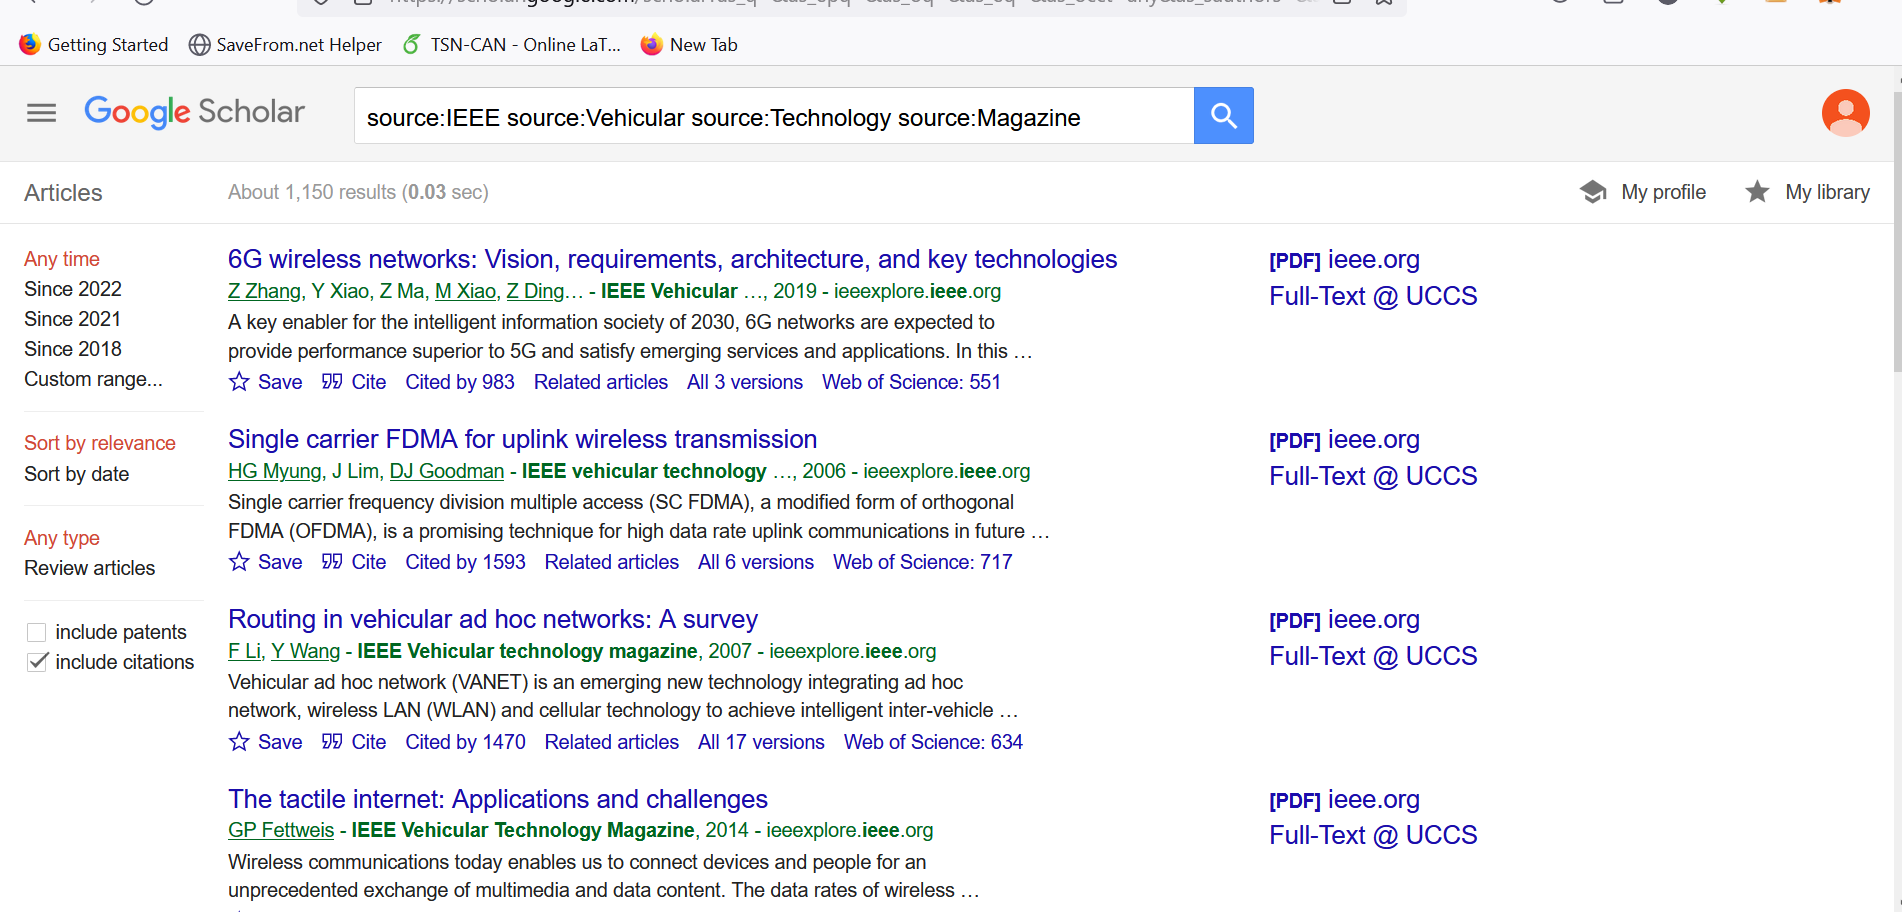
\includegraphics[width=0.9\textwidth]{Screenshot (282).png}
  \caption{Google Scholar.}
  \label{fig:google}
  \end{figure}
  
\begin{figure}[htbp]
  \centering
  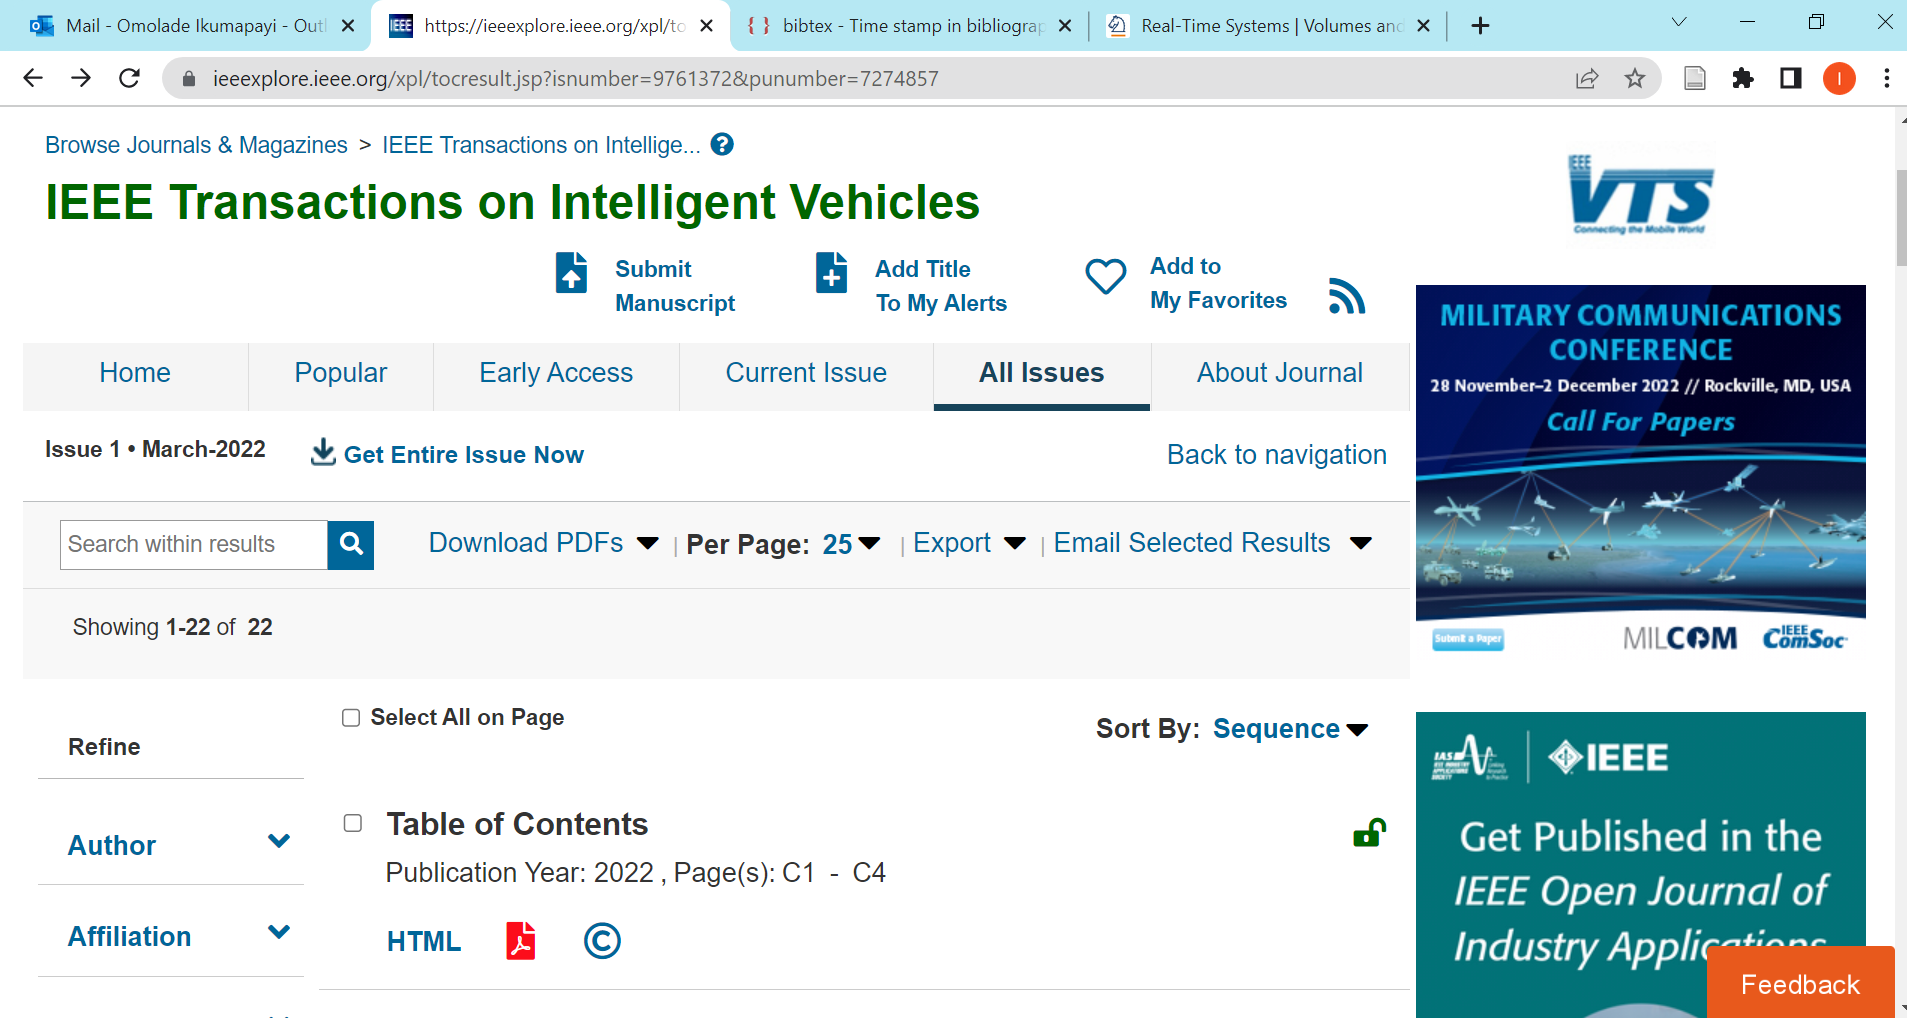
\includegraphics[width=0.9\textwidth]{Screenshot (280).png}
  \caption{Venue.}
  \label{fig:venue}
  \end{figure}
Figure \ref{fig:venue} shows the venue \cite{conference} I chose, the venue has different issues (up to 25) in a year and has about 25 papers in each issues making $>$ 50 papers per year. I chose this venue because I have been interested in the state-of-the-art technologies in vehicles, especially with the advent of the advanced driver assistance (ADAS), Vehicle to everything (V2X) and unmanned vehicle technology. I intend to have a knowledge of how different parts of a car are being automated and the advancement researchers have made in the past years and the mechanism around the automated vehicles 
\cite{9761719}

\begin{figure}[t!]
  \centering
  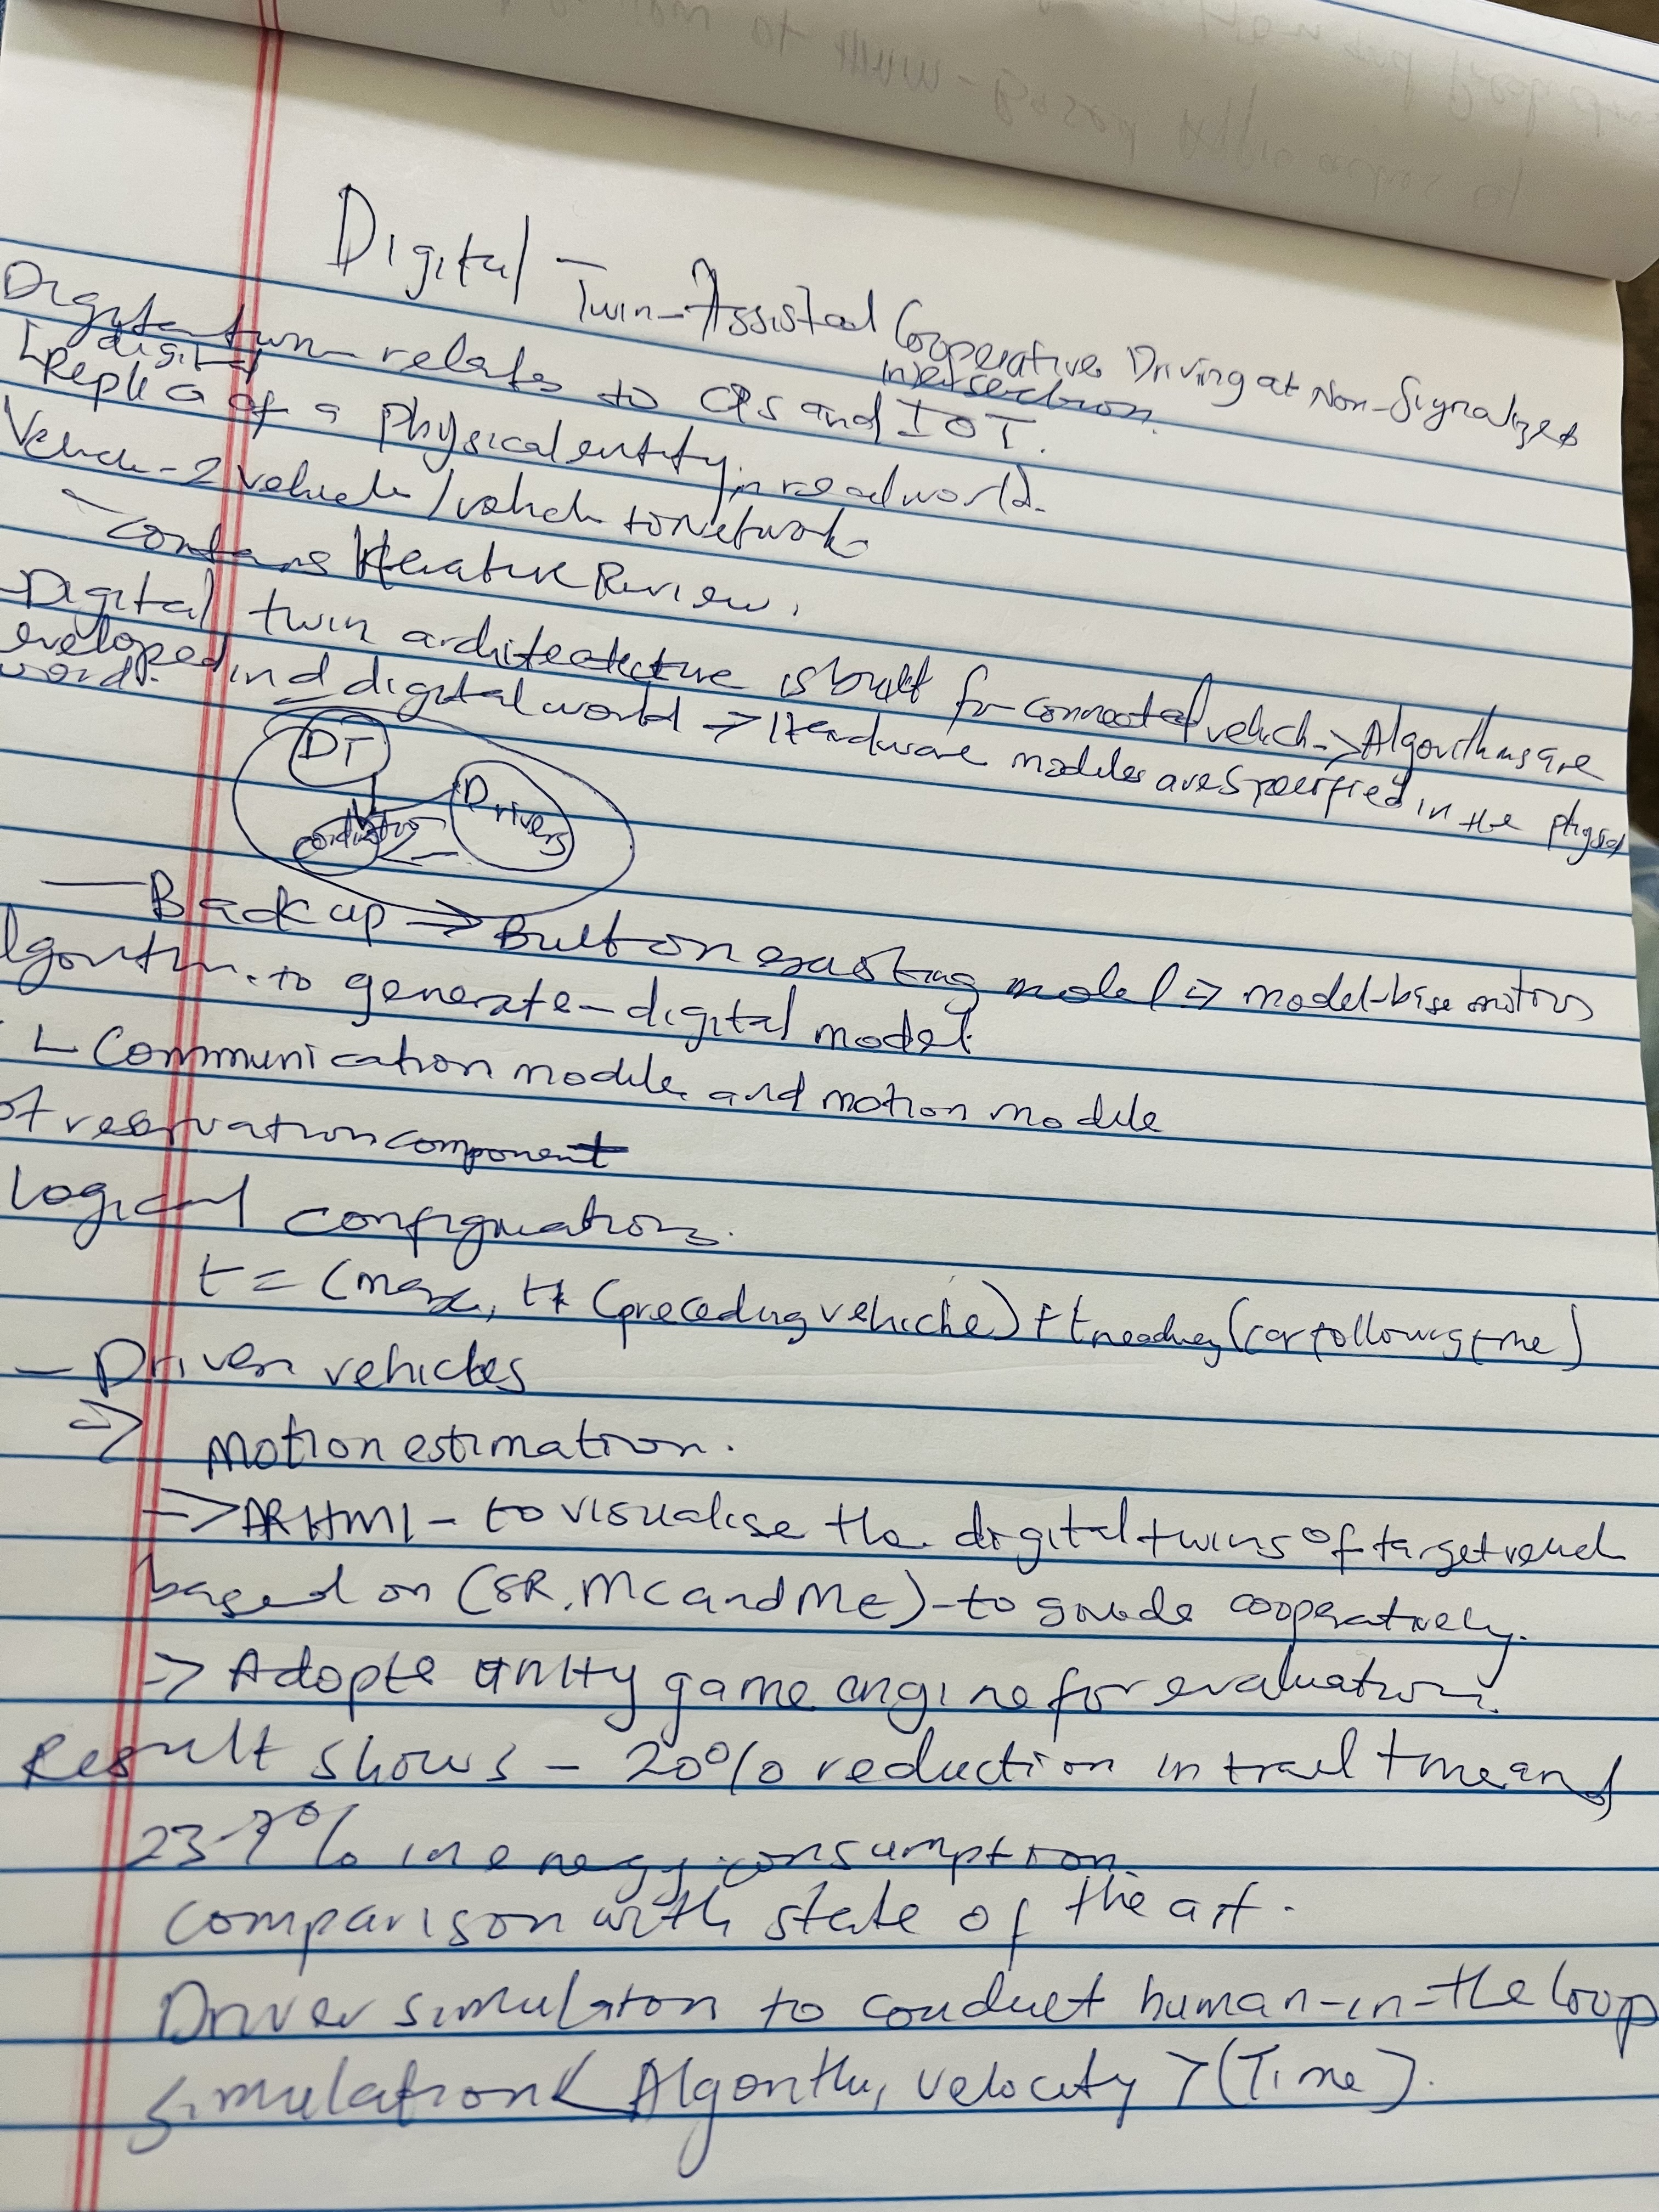
\includegraphics[width=1\textwidth]{IMG-8416.jpg}
  \caption{Note.}
  \label{fig:digital}
  \end{figure}
  
\begin{figure}[htbp]
  \centering
  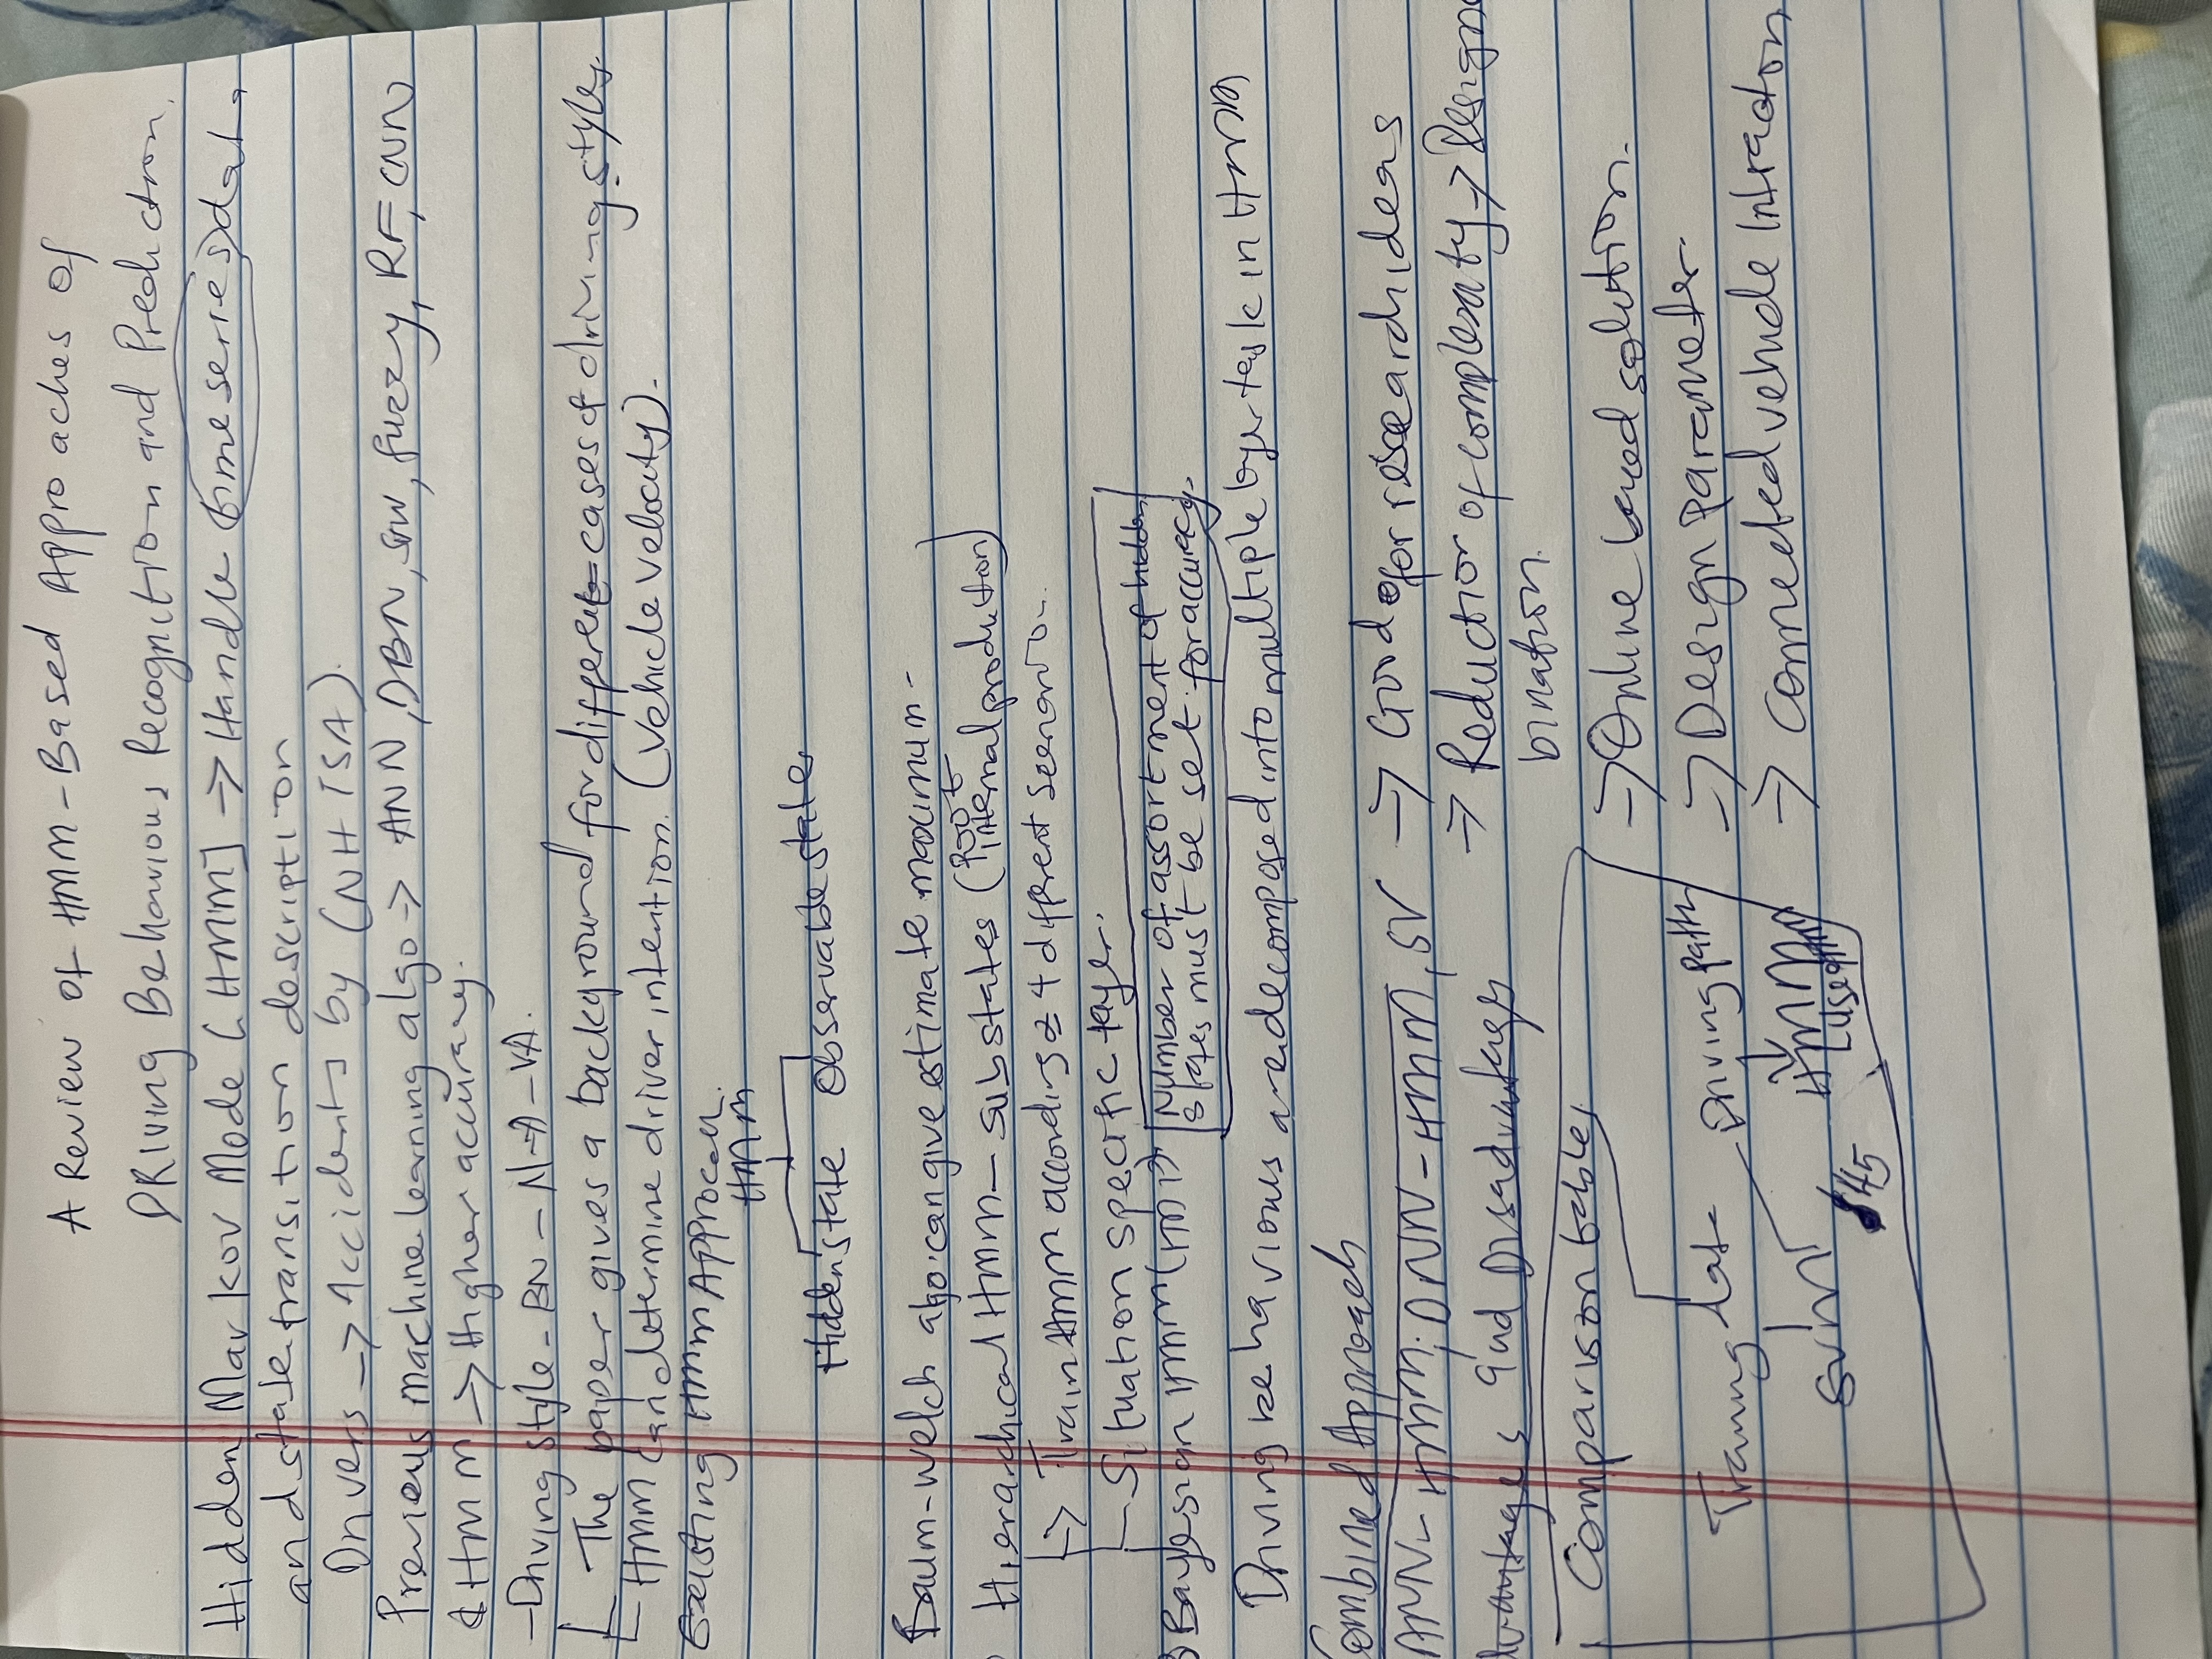
\includegraphics[width=1.2\textwidth,angle= 270]{IMG-8414.jpg}
  \caption{Note.}
  \label{fig:review}
  \end{figure}
\section{Learning Process}
The first challenge was to understand how to search for venue (IEEE Transactions of intelligent vehicles), since I am used to searching for keywords on google scholar. I went through google scholar search engine for my desired venue, then I found myself at the table of content page for the venue. While browsing through the issues, many of the papers were not exactly what I was looking for, as I was hoping to have background details into intelligent vehicles, however, some are survey papers and I gained handful knowledge. I realised I spent more time browsing the survey papers as I got too engrossed and I had to tell myself to wait till the scanning phase. For the scanning phase, I spent time understanding the methodology used in the eight papers I chose and for the critical and creative reading, I was able to read and get what I was looking for. The reason for the choice of the first paper is that it contains good ideas for future work after the review they did, and they have a comparison table to differentiate what others had done before. For the second paper, it was perfect for this area of research with detailed experiment.
Finally, it was not as easy as I was expecting especially filling in the notes and summary in the bibtex.

\section{Creative and Critical read}
\subsection{A review of HMM-Based Approaches of driving behaviour Recognition and Prediction} 
Problem was carefully stated and formulated. They did not test results from previous studies, however, a review from another paper that did this was included, they included comparison table and combination of algorithm, their survey is straightforward and someone new to the topic can read this paper and be well-informed on the state of the art. Well explained and detailed. Research ideas are well presented in this paper. Fig \ref{fig:review} shows my note from this paper.
\subsection{Digital Twin Assisted Cooperative Driving at Non-Signalized Intersection} This paper provides a good model to simulate their proposal, feasible experiments, enhanced solution that does motion estimation in a non-signalized intersection. Although I still feel that it is not the best solution and can be improved, (20$\%$ reduction), and that different driving laws can affect their solution, however, evaluation and implementation with real cases is good. Fig \ref{fig:digital} shows my note from this paper

Other Papers includes:
\cite{9068410},\cite{9277572},\cite{9291414},\cite{9291433},\cite{9305274}, \cite{9310276},\cite{9314262}, \cite{9319548},\cite{9351650}, \cite{9359494},\cite{9362281},\cite{9366366},\cite{9368510}, \cite{9372802},\cite{9372805},\cite{9380511},\cite{9380554}, \cite{9380699},\cite{9381686},\cite{9384276},\cite{9384316},\cite{9409672},\cite{9427213},\cite{9437967},\cite{9445043},\cite{9478305},\cite{9484798},\cite{9497693},\cite{9511277},\cite{9536371},\cite{9560150},\cite{9580729},\\\cite{9591277},\cite{9591322},\cite{9625720},\cite{9670638},\cite{9678034},\cite{9684928},\cite{9689059},\cite{9693162},\cite{9693282},\cite{9696256},\cite{9712376},\cite{9743954},\cite{9761398},\cite{9761719},\cite{9809823},\cite{9815528},\cite{9826530},\cite{9826532}.\\
Link: \url{https://www.overleaf.com/project/631807f3bedd0e55d73cfcbd}
\bibliographystyle{IEEEtran}
\bibliography{bib/paper}
\end{document}
